\documentclass[english]{article}
\usepackage{graphicx}
\usepackage{amsmath}
\usepackage{hyperref}
\usepackage{setspace}
\usepackage{apacite}
\usepackage{natbib}
\usepackage{pxfonts}
\usepackage[utf8]{inputenc}
\usepackage[left=1in,right=1in,top=1in,bottom=1in]{geometry}
\usepackage[left]{lineno}
\linenumbers


\title{An examination of the high-order dynamic interactions
  underlying multi-dimensional timeseries data} \author{Lucy
  L. W. Owen$^1$, Thomas Hao Chang$^{1,2}$, and\
  Jeremy R. Manning\textsuperscript{$1, \dagger$}\\
  [0.1in]$^1$Department of Psychological and Brain
  Sciences,\\Dartmouth
  College, Hanover, NH\\
  $^3$Amazon.com, Seattle, WA\\
  \textsuperscript{$\dagger$}Address correspondence to
  jeremy.r.manning@dartmouth.edu}


\begin{document}
\maketitle

\begin{abstract}
  Most complex systems reflect dynamic interations between myriad
  evolving components (e.g., interacting molecules, interacting brain
  systems, interacting individuals within a social network or
  ecological system, coordinated components within a mechanical or
  digital device, etc.).  Despite that these interactions are central
  to the full system's behavior (e.g., removing a component from the
  full system can change the entire system's behavior), dynamic
  interactions cannot typically be directly measured.  Rather, the
  interactions must be inferred through their hypothesized role in
  guiding the dynamics of system components.  Here we use a
  model-based approach to inferring dynamic interactions from
  timeseries data.  In addition to examining first-order interactions
  (e.g., between pairs of components) we also examine higher-order
  interactions (e.g., that characterize mirrored structure in the
  patterns of interaction dynamics displayed by different subsets of
  components).  We apply our approach to two datasets.  First, we use
  a synthetic dataset, for which the underlying dynamic interactions
  are known, to show that our model recovers those ground-truth
  dynamic interactions.  We also apply our model to a neuroimaging
  dataset and show that the high-order dynamic interactions exhibited
  by brain data vary meaningfully as a function of the cognitive
  ``richness'' of the stimulus people are experiencing.
\end{abstract}

\doublespacing

\section*{Introduction}
The dynamics of the observable universe are meaningful in three
respects.  First, the behaviors of the \textit{atomic units} that
exhibit those dynamics are highly interrelated.  The actions of one
unit typically have implications for one or more other units.  In
other words, there is non-trivial \textit{correlational structure}
defining how different units interact with and relate to each other.
Second, that correlational structure is \textit{hierarchical} in the
sense that it exists on many spatiotemporal scales.  The way one group
of units interacts may relate to how another group of units interact,
and the interactions between those groups may exhibit some rich
structure.  Third, the structure at each level of this correlational
hierarchy changes from moment to moment, reflecting the ``behavior''
of the full system.

These three properties (rich correlations, hierarchical organization,
and dynamics) are major hallmarks of many complex systems.  For
example, within a single cell, the cellular components interact at
many spatiotemporal scales, and those interactions change according to
what that single cell is doing.  Within a single human brain, the
individual neurons interact within each brain structure, and the
structures interact to form complex networks.  The interactions at
each scale vary according to the functions our brains are carrying
out.  And within social groups, interactions at different scales
(e.g., between individuals, family units, communities, etc.) vary over
time according to changing goals and external constraints.

Although many systems exhibit rich dynamic correlations at many
scales, a major challenge to studying such patterns is that typically
neither the correlations nor the hierarchical organizations of those
correlations may be directly observed.  Rather, these fundamental
properties must be inferred indirectly by examining the observable
parts of the system-- e.g., the behaviors of the individual atomic
units of that system.  In the \textit{Methods} section, we propose a
series of mathematical operations that may be used to recover dynamic
correlations at a range of scales (i.e., orders of interaction).  In
the \textit{Results} section, we demonstrate how our approach may be
applied to multi-dimensional timeseries data: a synthetic dataset
where the underlying dynamic correlations are known (we use this
dataset to validate our approach), and a neuroimaging dataset
comprising data collected as participants listened to a
story~\citep{SimoEtal16}.  In different experimental conditions in the
neuroimaging study, participants listened to altered versions of the
story that varied in cognitive richness: the intact story (fully
engaging), a scrambled version of the story where the paragraphs were
presented in a randomized order (moderately engaging), a second
scrambled condition where the words were presented in a random order
(minimally engaging), and a ``rest'' condition where the participants
did not listen to any version of the story (control condition).  We
use the neuroimaging dataset to examine how higher-order structure in
brain data varies as a function of the cognitive richness of the
stimulus.

\section*{Methods}
There are two basic steps to our approach.  In the first step, we take
a number-of-timepoints ($T$) by number-of-features ($F$)
\textit{matrix of observations} ($\mathbf{X}$) and we return a $T$ by
$\frac{F^2 - F}{2}$ \textit{matrix of dynamic correlations}
($\mathbf{Y}$).  Here $\mathbf{Y_0}$ describes, at each moment, how
all of the features (columns of $\mathbf{X}$) are inferred to be
interacting.  (Since the interactions are assumed to be non-recurrent
and symmetric, only the upper triangle of the full correlation matrix
is computed.)  In the second step, we project $\mathbf{Y_0}$ onto an
$F$-dimensional space, resulting in a new $T$ by $F$ matrix
$\mathbf{Y_1}$.  Note that $\mathbf{Y_1}$ contains information about
the correlation dynamics present in $\mathbf{X}$, but represented in a
compressed number of dimensions.  By repeatedly applying these two
steps in sequence, we can examine and explore higher order dynamic
correlations in $\mathbf{X}$.

\subsection*{Dynamic correlations}
Given a matrix of observations, we can compute the (static)
correlations between any pair of observations, $\mathbf{X}_i$ and
$\mathbf{X}_j$ using:
\begin{align}
  \mathrm{corr}(\mathbf{X}_i, \mathbf{X}_j) &= \frac{\sum_{t=1}^T \left(\mathbf{X}_i(t)
                                              -
                                              \hat{\mathbf{X}_i}\right) \left(\mathbf{X}_j(t)
                                              -
                                              \hat{\mathbf{X}_j}\right)}{\sqrt{\sum_{t=1}^T\left(
                                              \sigma^2_{\mathbf{X}_i}\right) \left(
                                              \sigma^2_{\mathbf{X}_j}\right)}},~\mathrm{where}\\
                                    \hat{\mathbf{X}_k} &= \sum_{t=1}^T
                                                         \mathbf{X}_k(t),~\mathrm{and}\\
  \sigma^2_{\mathbf{X}_k} &= \sum_{t=1}^T \left( \mathbf{X}_k -
                            \hat{\mathbf{X}_k} \right)^2 
\end{align}

We can generalize this formula to compute time-varying correlations by
incorporating a \textit{weight function} that takes a time $t$ as input,
and returns how much the observed data every timepoint (including $t$)
contribute to the correlations at time $t$ (Fig.~\ref{fig:weights}).
\begin{figure}
  \centering
  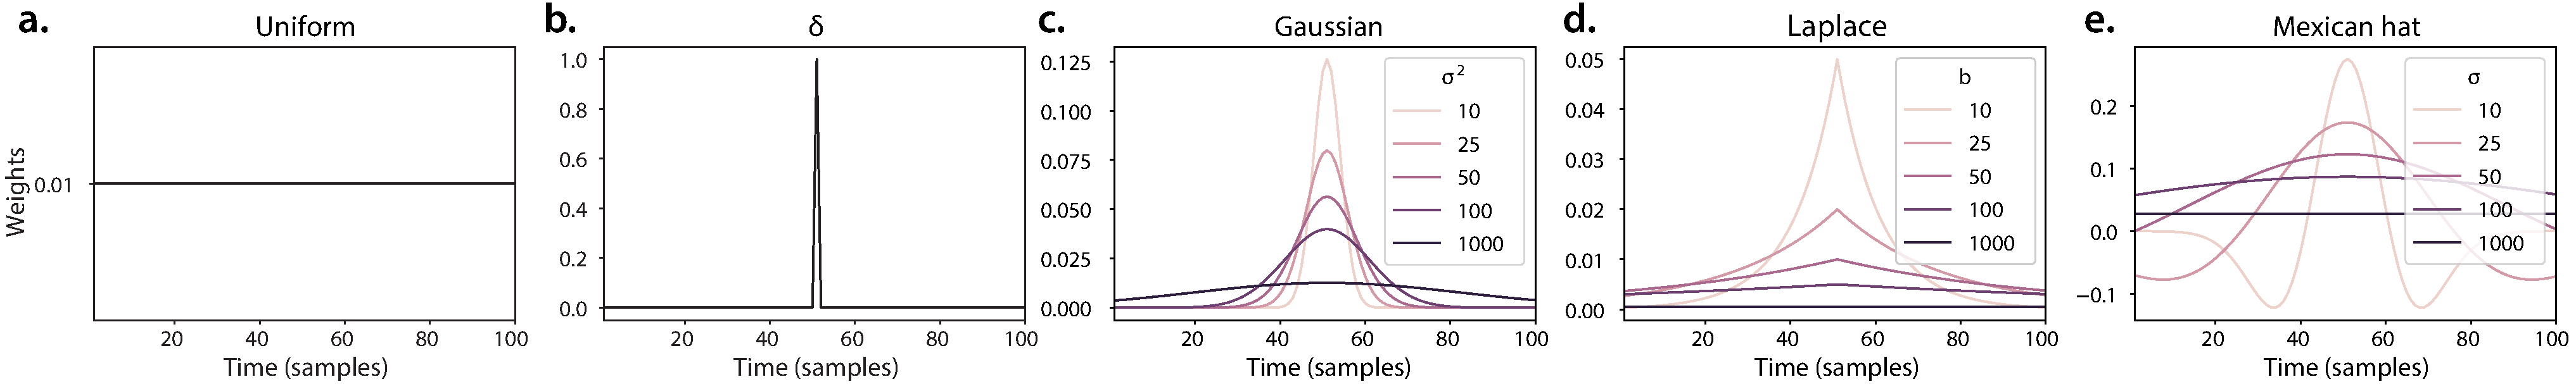
\includegraphics[width=\textwidth]{figs/kernels}
  \caption{\textbf{Examples of time-varying weights.  Each panel
    displays per-timepoint weights computed for 100 timepoints
    ($0, 1, ..., 99$) with $t = 50$.  a. Uniform weights.} The weights
  are timepoint-invariant; all timepoints are weighted equally, and do
  not change as a function of $t$.  This is a special case of weight
  function that reduces dynamic correlations to static correlations.
  \textbf{b. Dirac delta function.} Only the timepoint $t$ is given
  weight (of 1), and all other timepoints' weights are set to 0.
  \textbf{c. Gaussian weights.} Each timepoint's weights fall off
  according to a Gaussian probability density function centered on
  $\mu = t$.  Weights derived using several different example variance
  parameters ($\sigma^2$ are displayed.  \textbf{d. Laplace weights.}
  Each timepoint's weights fall off according to a Laplace probability
  density function centered on $\mu = t$.  Weights derived using
  several different example scale parameters ($b$) are displayed.}
  \label{fig:weights}
\end{figure}

%include figure showing weights (https://github.com/ContextLab/timecorr-paper/issues/1)

\textbf{JRM STOPPED HERE}
\begin{align}
\mathrm{corr}_t(x,y) &= \frac{\sum_{t=1}^T \left( x_t - \bar{x_t} \right) \left( y_t - \bar{y_t} \right)}{\sqrt{\sum_{t=1}^{T}\sigma ^{2}_{x_{t}}\sigma ^{2}_{y_{t}}}}\mathrm{, where}\\
\bar{a_t} &= \sum_{t=1}^T w(t)_i a_i\\
\sigma^{2}_{a_t} &= \sum_{t=1}^{T} \left(a_t - \bar{a_t} \right)^2\\
w(t) &= \mathcal{N}\left(1...T ~|~ t, \sigma_\mathcal{N}\right) %update to include eye, laplace, and gaussian weights
\end{align}



% \begin{equation}
% c(t) = \sum_{i=1}^{T}w(t)_{i}
% \end{equation}



\section*{Results}
%currently Lucy, Kirsten, and Paxton have agreed to make figures

%%%%%%%%%%%%%%%%%%%%%%%%%%%%%%%%%%%%%%%
\section*{Discussion}
% multiple timescale representations (a la Hasson group) implies
% first-order network interactions.  higher-order interactions imply
% generalizations between interacting representations (e.g. mirrored
% schema, a la Norman/Baldassano/Hasson).  possibly cite NTB 2013
% science review, using as evidence that this is where the field is
% going (voxels --> patterns (L0) --> interactions (L1) --> higher
% order patterns (L2+).

% related approaches: sliding window, phase-based correlations,
% within-ROI spatial correlations at each timepoint, granger
% causality, other explit models (e.g. virtual brain).

%other applications: molecular interactions (protein folding?),
%diagnosis (e.g. psychiatric disorders as network flow problems--
%gratton work?), social network dynamics (e.g. financial markets,
%social media interactions)

\subsection*{Concluding remarks}
% the universe is complicated and we need scalable approaches to
% studying how the pieces are interacting to make sense of it.  one
% small step for mankind, and so on.

\section*{Acknowledgements}
We acknowledge discussions with Luke Chang, Hany Farid, Paxton
Fitzpatrick, Andrew Heusser, Eshin Jolly, Qiang Liu, Matthijs van der
Meer, Judith Mildner, Gina Notaro, Stephen Satterthwaite, Emily
Whitaker, Weizhen Xie, and Kirsten Ziman. Our work was supported in
part by NSF EPSCoR Award Number 1632738 to J.R.M. and by a sub-award
of DARPA RAM Cooperative Agreement N66001-14-2-4-032 to J.R.M.  The
content is solely the responsibility of the authors and does not
necessarily represent the official views of our supporting
organizations.

\section*{Author contributions}
Concept: J.R.M.  Implementation: T.H.C., L.L.W.O., and
J.R.M.  Analyses: L.L.W.O and J.R.M.

\bibliographystyle{apacite}
\bibliography{CDL-bibliography/memlab}

\end{document}

